
\section{Preliminary experiments}
Here we describe one numerical simulation from each code to give a
qualitative picture of disc evolution. In the next section, we analyse
2D simulations in more detail and explore parameter space.  

In these simulations we subject the disc to random perturbations in
cylindrical velocity,
\begin{align}\label{randpert}
  \frac{\delta v_R}{c_s} = \frac{\delta}{M}\times T(R) \sum_{m=1}^M\cos{m\phi},
\end{align}
where $\delta\in[-10^{-3},10^{-3}]$ is chosen randomly but does not
depend on $\phi$, and 
\begin{align}
  T(R) =
  \exp{\left[-\frac{1}{2}\left(\frac{R-\overline{R}_d}{\Delta
          R_d}\right)^2\right]}, 
\end{align}
where $\overline{R}_d = (R_{d1}+R_{d2})/2$ and $\Delta R_d =
(R_{d2}-R_{d1})/2$. 
\subsection{FARGO 2D}\label{fargo_fiducial}
We consider a disc size $[R_\mathrm{min}, R_\mathrm{max}] =
[0.4,10]R_0$ and resolution $N_R\times N_\phi = 512\times 1024$ or
about $8$ grids per $H$. We adopt $\epsilon_g=10^{-4}H$ for the 
self-gravity softening length\footnote{In 2D self-gravity, $\epsilon_g$ also
  approximates for the vertical disc thickness, so a more appropriate
  value would be $\epsilon_g\sim H$ \citep{muller12}. However, because
  $\epsilon_g\propto R$ is needed in FARGO, the Poisson kernel
  (Eq. \ref{2d_grav}) is no longer symmetric in $(R,R^\prime)$. We
  choose a small  
  $\epsilon_g$ in favour of angular momentum conservation, keeping in
  mind that the strength of self-gravity will be over-estimated.}, and 
set $M=10$ for random perturbations (Eq. \ref{randpert}). 

Snapshots from the disc evolution is shown in Fig. \ref{fargo_2d} in
terms of the non-axisymmetric surface density. 


\begin{figure}
  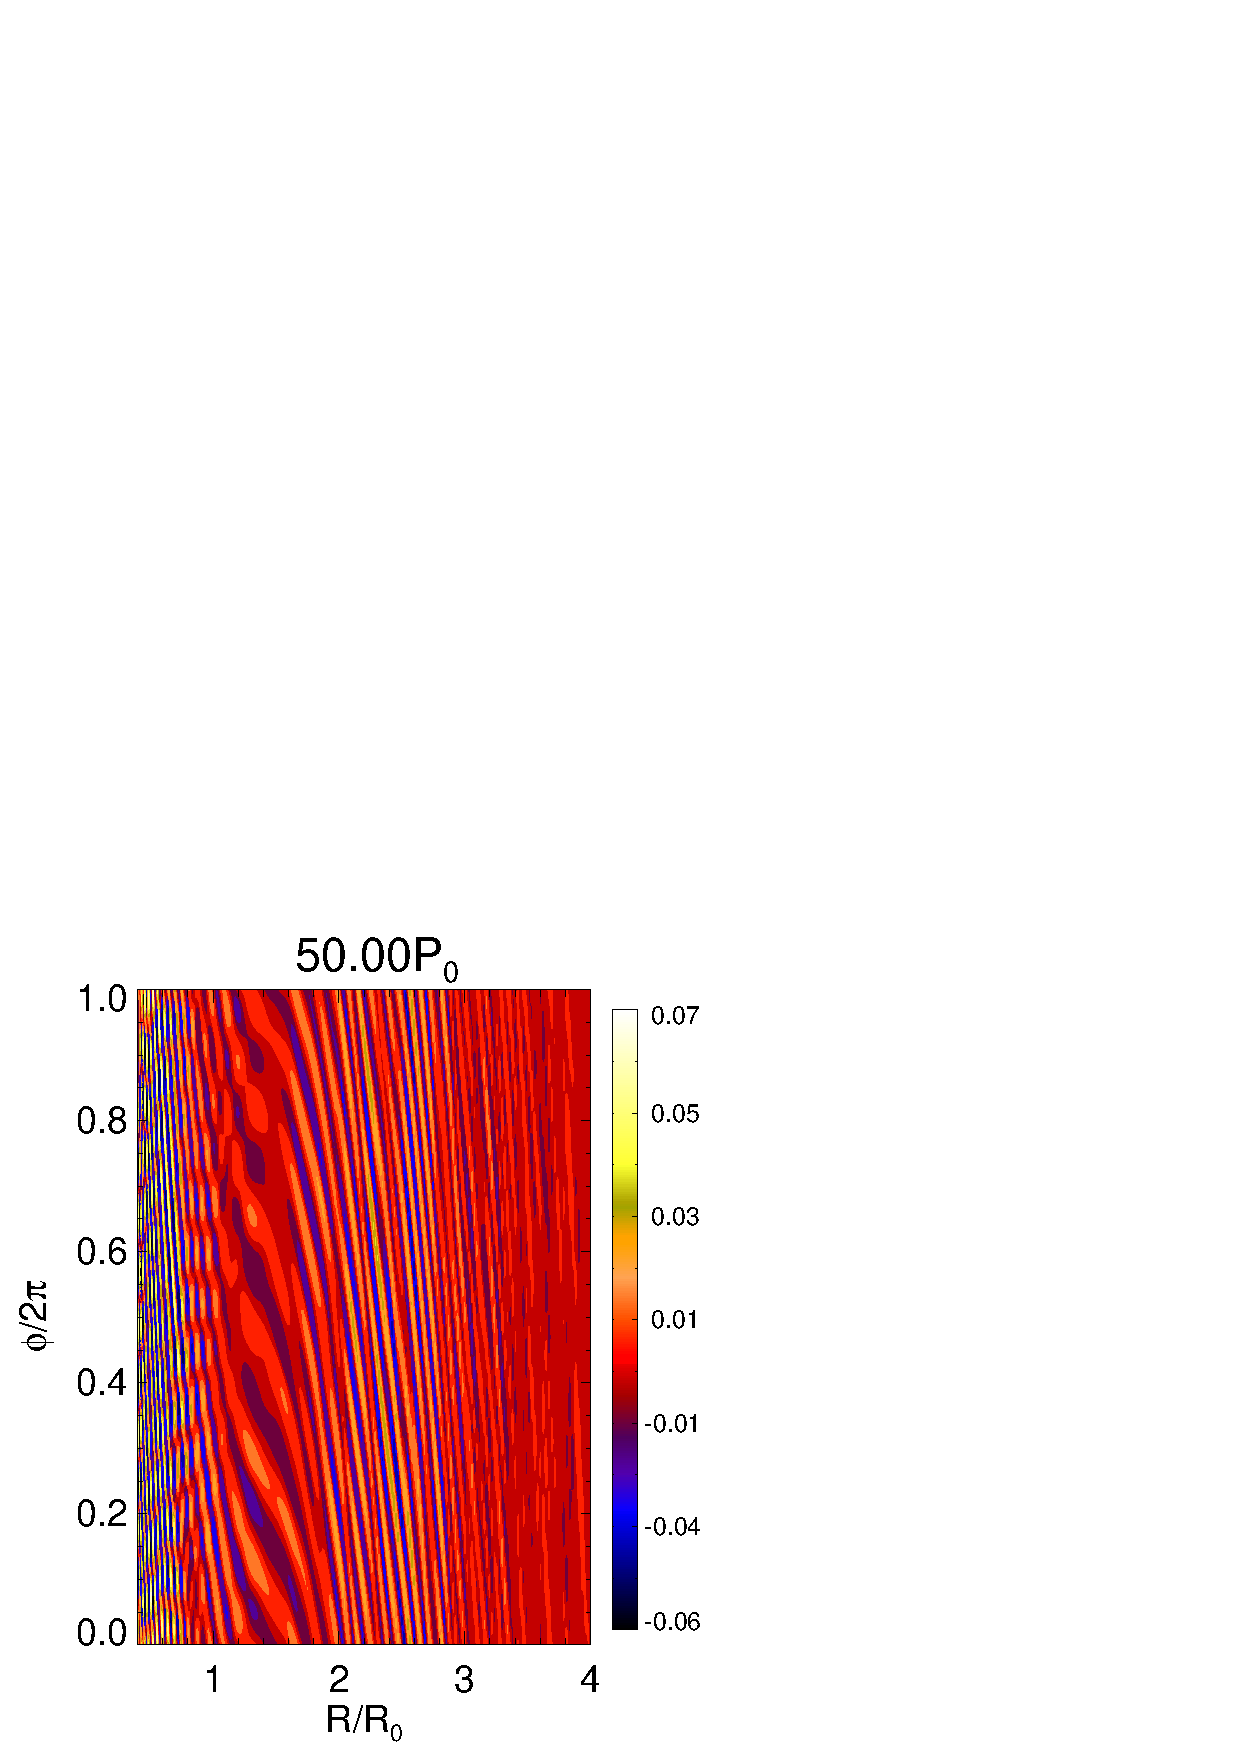
\includegraphics[scale=0.27]{figures/polarxy_dens050}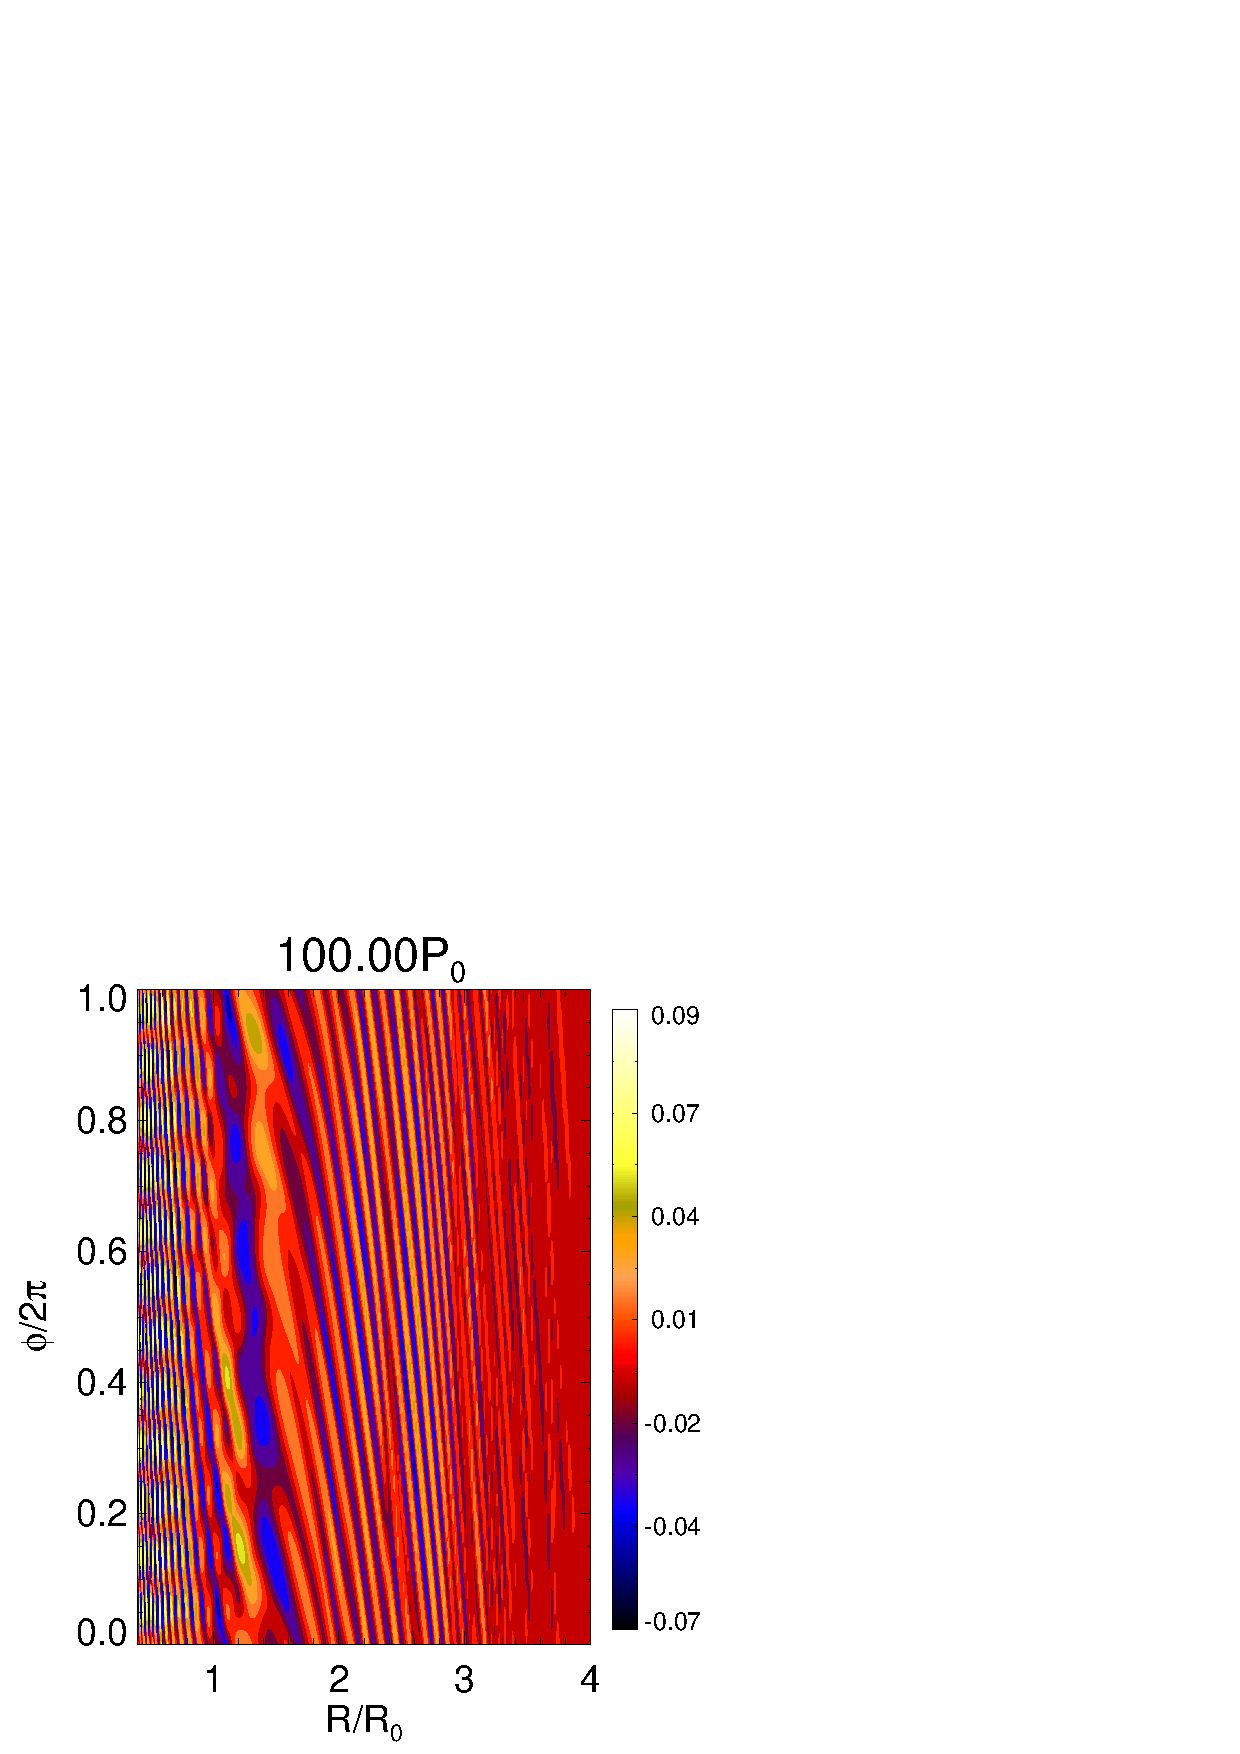
\includegraphics[scale=0.27,clip=true,trim=2.26cm 
  0cm 0cm
  0cm]{figures/polarxy_dens100}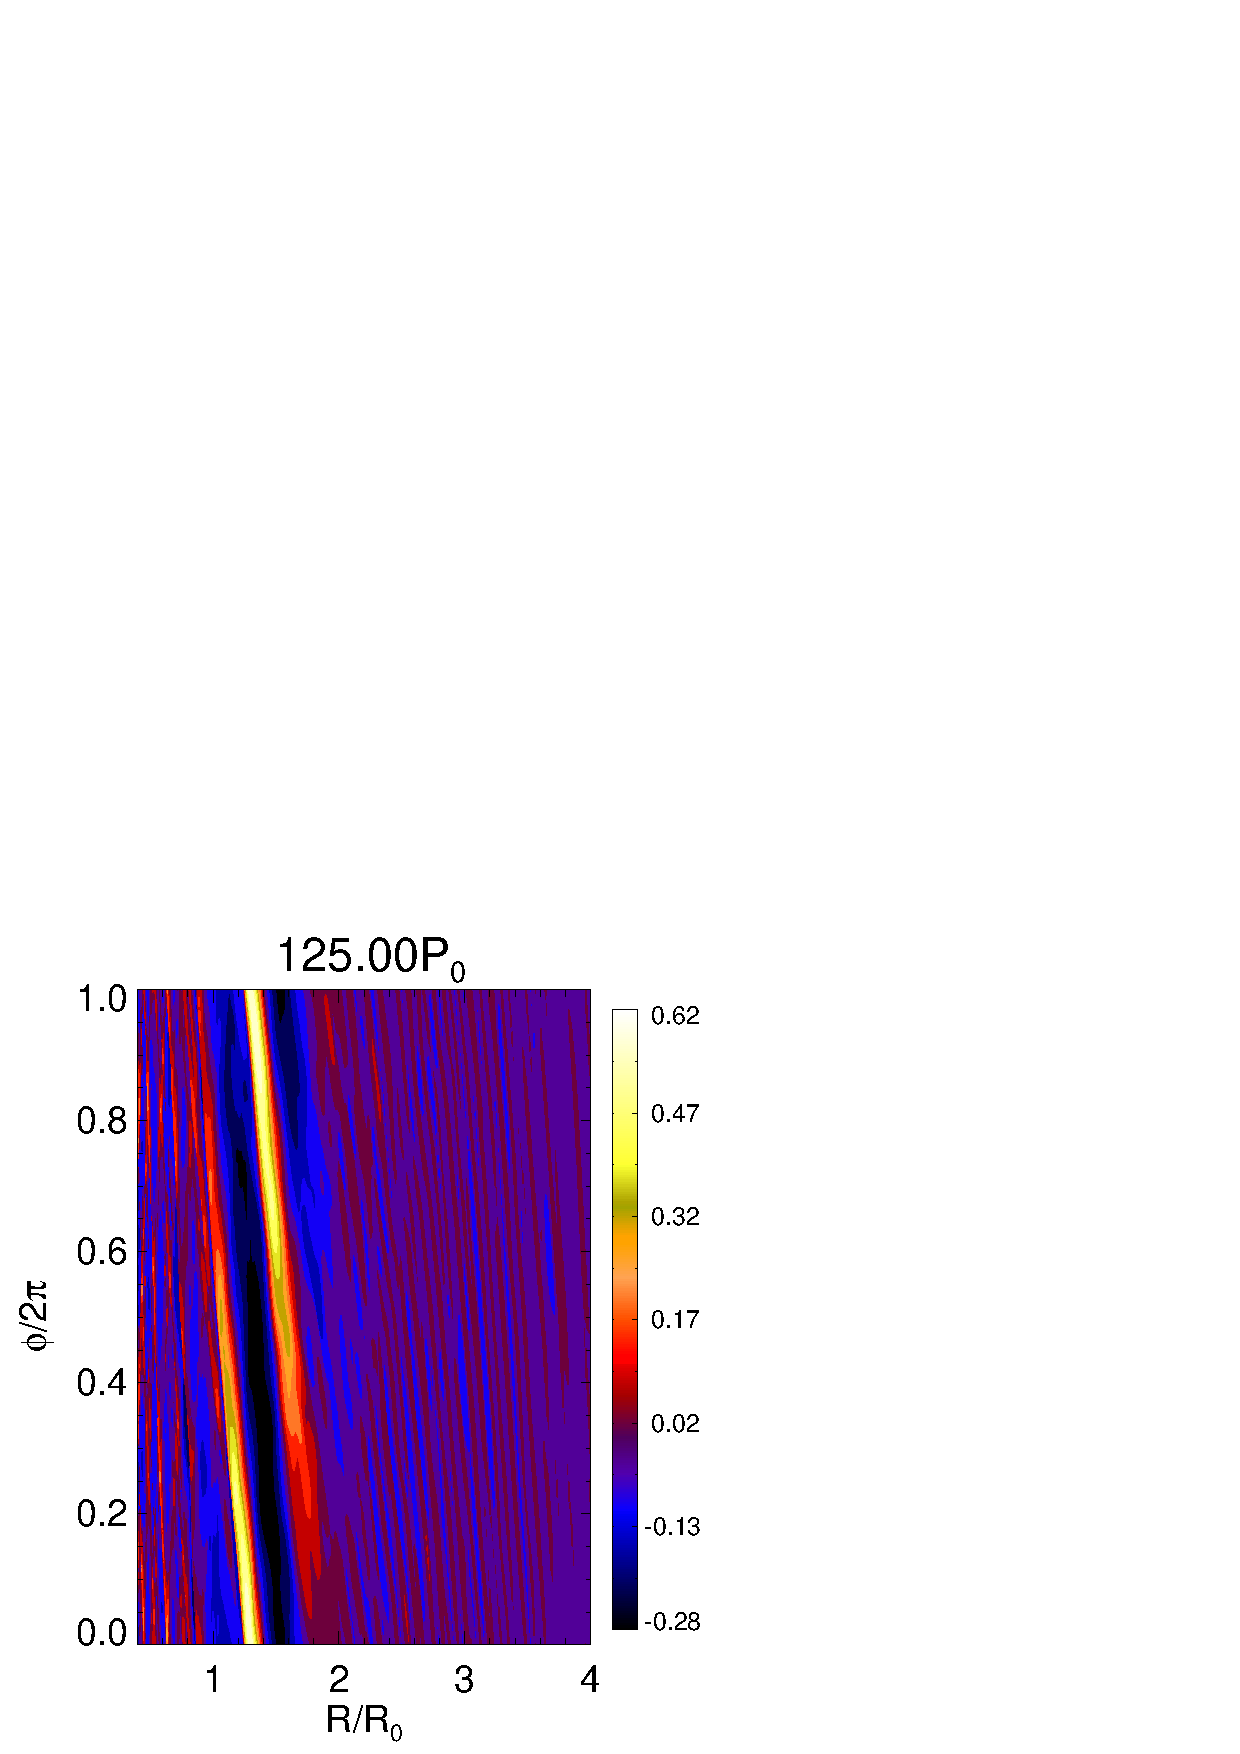
\includegraphics[scale=0.27,clip=true,trim=2.26cm
  0cm 0cm 0cm]{figures/polarxy_dens125} 
  \caption{Fiducial FARGO 2D simulation (\S\ref{fargo_fiducial}),
    showing the evolution of the non-axisymmetric surface density
    $\Delta\Sigma$. Note that the disc extends to $R=10R_0$, but only
    the inner part is shown for clarity. \label{fargo_2d}} 
\end{figure}

\begin{figure}
  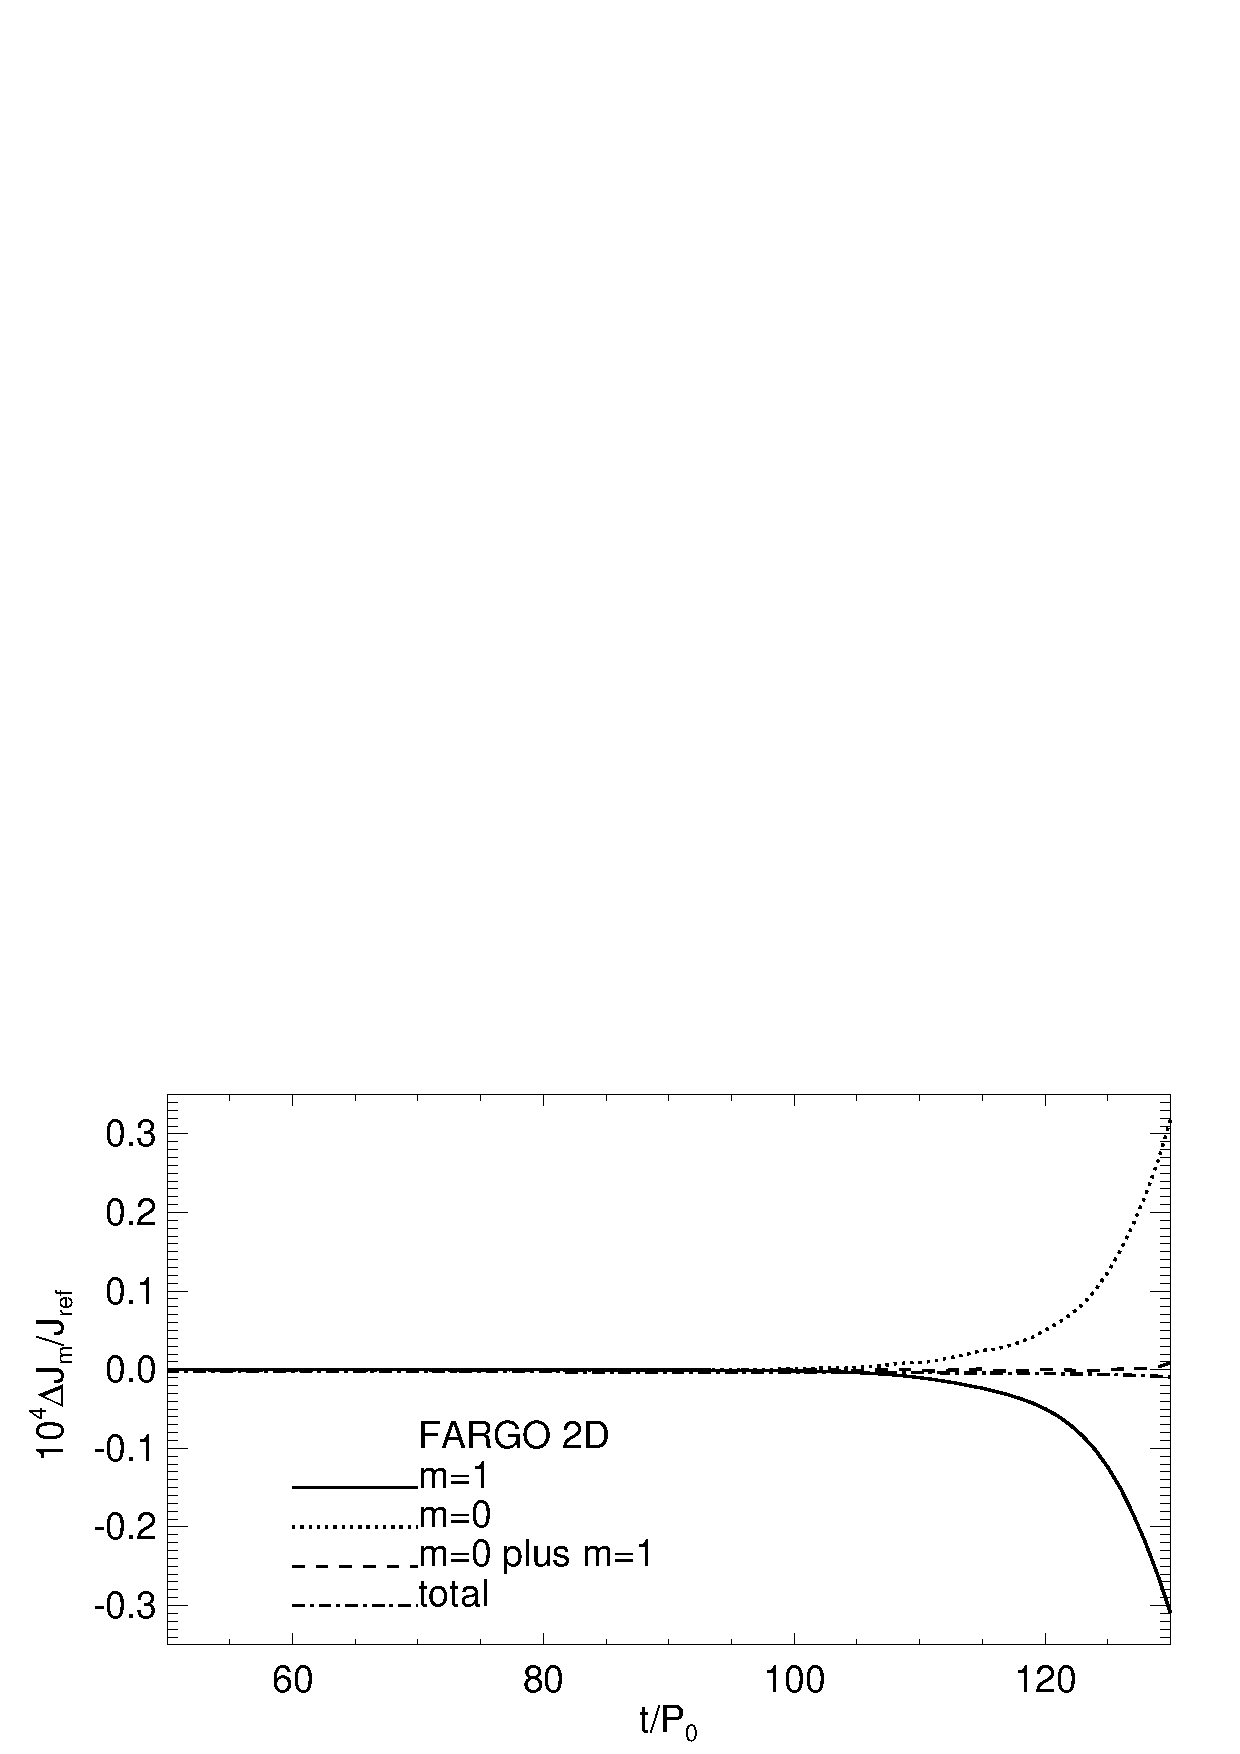
\includegraphics[width=\linewidth]{figures/nonaxi_evol_ang_fargo}
  \caption{Evolution of angular momentum components in the FARGO
    fiducial simulation (Fig. \ref{fargo_2d}). The perturbation
    relative to $t=0$ is shown in units of the initial total angular
    momentum $J_\mathrm{ref}$.\label{fargo_2d_angmom}} 
\end{figure}

\subsection{ZEUS-MP 3D}





\subsection{PLUTO 3D}





